\clearpage
\maketitlesupplementary

\renewcommand{\thesection}{S\arabic{section}}
\setcounter{section}{0}
\renewcommand{\theequation}{S\arabic{equation}}
\setcounter{equation}{0}
\renewcommand{\thetable}{S\arabic{table}}
\setcounter{table}{0}
\renewcommand{\thefigure}{S\arabic{figure}}
\setcounter{figure}{0}

This supplementary material gives the proofs deferred from \Cref{sec:method} (\Cref{sec:supp_taylor,sec:supp_adjoint}) and an additional qualitative figure (\Cref{sec:supp_qual}).

\section{Proof of \Cref{prop:decomposition} (Backbone Dominance)}
\label{sec:supp_taylor}

Write $\theta_0=(\theta_0^b,\theta_0^h)$ and $L(\phi):=\mathbb{E}_{Q_i}[\mathcal{L}(Q_i,\phi)]$, twice continuously differentiable in a neighborhood containing $\theta_0$ and the full trajectory. Let $g_b,g_h,H_{bb},H_{bh},H_{hh}$ be the gradient/Hessian blocks of $L$ at $\theta_0$, and $\Delta b_T:=\phi_T^b-\theta_0^b$, $\Delta h_T:=\phi_T^h-\theta_0^h$, $\Delta h_T^f:=\phi_T^{f,h}-\theta_0^h$ (the frozen branch has $\Delta b_T^f=0$ by construction).

\paragraph{Second-order expansion.} Expanding $L$ to second order around $\theta_0$ along each branch and subtracting (the $L(\theta_0)$ terms cancel) reproduces \Cref{eq:decomposition} exactly, with $C_b$ collecting every term touched by $\Delta b_T$ and $R_h$ the rest.

\begin{lemma}[Displacement is $O(T\alpha)$]
\label{lem:displacement}
If $\|\nabla_\phi\mathcal{L}(\phi,S_i)\|\le G$ along the trajectory, then $\|\Delta b_T\|,\|\Delta h_T\|,\|\Delta h_T^f\|=O(T\alpha)$.
\end{lemma}
\begin{proof}
Each inner-loop step moves the parameters by at most $\alpha G$ (\Cref{eq:inner_loop}); summing $T$ steps via the triangle inequality bounds the total displacement by $T\alpha G$, for both branches and both parameter blocks.
\end{proof}

\begin{lemma}[Head divergence is $O((T\alpha)^2)$]
\label{lem:head_div}
Let $\delta_j:=\Delta h_j-\Delta h_j^f$. If $\nabla_h\mathcal{L}(\cdot,S_i)$ is $L$-Lipschitz in $\phi$, then $\delta_1=0$ exactly, and $\delta_T=O((T\alpha)^2)$.
\end{lemma}
\begin{proof}
At $j{=}1$ both branches share $\phi_0=\phi_0^f=\theta_0$, so their first head-gradient step coincides exactly: $\delta_1=0$. For $j\ge2$, $\delta_j=\delta_{j-1}-\alpha[\nabla_h\mathcal{L}(\phi_{j-1},S_i)-\nabla_h\mathcal{L}(\phi_{j-1}^f,S_i)]$; the two arguments differ by $\Delta b_{j-1}=O((j{-}1)\alpha)$ in the backbone (\Cref{lem:displacement}) and $\delta_{j-1}$ in the head, so Lipschitzness gives $\|\delta_j\|\le(1{+}\alpha L)\|\delta_{j-1}\|+O((j{-}1)\alpha^2)$. Unrolling from $\delta_1=0$ under $T\alpha\ll1$ (Assumption~\ref{asm:fast_adaptation}, so $(1+\alpha L)^{T}=1+O(T\alpha)$ stays bounded) gives $\|\delta_T\|\le O(\alpha^2)\sum_{k=1}^{T-1}k\cdot(1+O(T\alpha))=O(\alpha^2T^2)=O((T\alpha)^2)$.
\end{proof}

\noindent\textbf{Conclusion.} By \Cref{lem:displacement}, $C_b$'s linear term $g_b^\top\Delta b_T$ is $O(T\alpha)$ and dominates its own quadratic terms, so $C_b=O(T\alpha)$. By \Cref{lem:head_div}, $R_h$'s linear term $-g_h^\top\delta_T$ and its quadratic terms are all $O((T\alpha)^2)$. Hence $\Delta M=-C_b+O((T\alpha)^2)$, proving \Cref{prop:decomposition}. At $T{=}1$, $\delta_1{=}0$ exactly, so $R_h{=}0$ exactly (not merely to leading order).

\section{Adjoint Equivalence and Stability}
\label{sec:supp_adjoint}

\begin{proposition}[Exactness of the adjoint recursion]
\label{prop:supp_exact}
The sequence $\{\lambda_t\}$ defined by \Cref{eq:adjoint_recursion} satisfies $\lambda_t=\partial L(\phi_T)/\partial\phi_t$ for every $t=0,\dots,T$, with no approximation beyond \Cref{eq:inner_loop} itself.
\end{proposition}
\begin{proof}
By backward induction on $t$. \emph{Base case} ($t{=}T$): by definition, $\lambda_T=\nabla_\phi L(\phi_T)=\partial L(\phi_T)/\partial\phi_T$. \emph{Step}: assume $\lambda_t=\partial L(\phi_T)/\partial\phi_t$. Since $\phi_T$ depends on $\phi_{t-1}$ only through $\phi_t$, the chain rule and the step-Jacobian $\partial\phi_t/\partial\phi_{t-1}=I-\alpha H_{t-1}$ (\Cref{eq:step_jacobian}, exact since \Cref{eq:inner_loop} is a literal function, not a discretized ODE) give $\partial L(\phi_T)/\partial\phi_{t-1}=(I-\alpha H_{t-1})^\top\lambda_t$. $H_{t-1}$ is a Hessian, hence symmetric, so this equals $\lambda_t-\alpha H_{t-1}\lambda_t=\lambda_{t-1}$ by \Cref{eq:adjoint_recursion}, completing the induction.
\end{proof}
Summing $\partial\Psi_t/\partial S_i\big|_{\phi_{t-1}}$ (the direct-dependence Jacobian of one inner-loop step on $S_i$) contracted with $\lambda_t$ over $t=1,\dots,T$, via the total-derivative rule for a parameter shared across a chain of composed functions, yields \Cref{eq:trajectory_expansion} directly from \Cref{prop:supp_exact}.

\begin{proposition}[Non-expansiveness]
\label{prop:supp_nonexpansive}
If $\alpha\le 2/\lambda_{\max}(H_{t-1})$ for every $t$, then $\|\lambda_{t-1}\|\le\|\lambda_t\|$, so $\{\lambda_t\}$ cannot blow up over $T$ backward steps.
\end{proposition}
\begin{proof}
$H_{t-1}$ is symmetric, hence orthogonally diagonalizable with real eigenvalues $\mu_i\in[\lambda_{\min},\lambda_{\max}]$. The stated bound on $\alpha$ gives $\alpha\mu_i\in[0,2]$, so every eigenvalue $1-\alpha\mu_i$ of $I-\alpha H_{t-1}$ lies in $[-1,1]$, i.e.\ $\|I-\alpha H_{t-1}\|_{\mathrm{op}}\le1$. Then $\|\lambda_{t-1}\|=\|(I-\alpha H_{t-1})\lambda_t\|\le\|\lambda_t\|$ follows directly from \Cref{eq:adjoint_recursion}.
\end{proof}

\begin{proposition}[Error accumulates linearly, not exponentially]
\label{prop:supp_error}
If every Monte Carlo-estimated HVP in \Cref{eq:adjoint_recursion} has error at most $\varepsilon$, then the backward pass accumulates total error $\|\hat\lambda_0-\lambda_0\|\le T\alpha\varepsilon$.
\end{proposition}
\begin{proof}
Let $e_t:=\hat\lambda_t-\lambda_t$ (with $e_T=0$). From the approximate and exact recursions, $e_{t-1}=(I-\alpha H_{t-1})e_t-\alpha(\widehat{H_{t-1}\lambda_t}-H_{t-1}\lambda_t)$; taking norms and using \Cref{prop:supp_nonexpansive} gives $\|e_{t-1}\|\le\|e_t\|+\alpha\varepsilon$. Unrolling from $e_T=0$ over $T$ steps gives $\|e_0\|\le T\alpha\varepsilon$.
\end{proof}
\Cref{prop:supp_error} means the bootstrap sample count controlling $\varepsilon$ (\Cref{sec:fama}) need only scale to keep $\varepsilon$ small, not to compensate for exponential blow-up across $T$ -- consistent with the fast-adaptation regime ($T\alpha\ll1$) that Assumption~\ref{asm:fast_adaptation} already assumes.

\section{Additional Qualitative Example}
\label{sec:supp_qual}

\begin{figure*}[t]
    \centering
    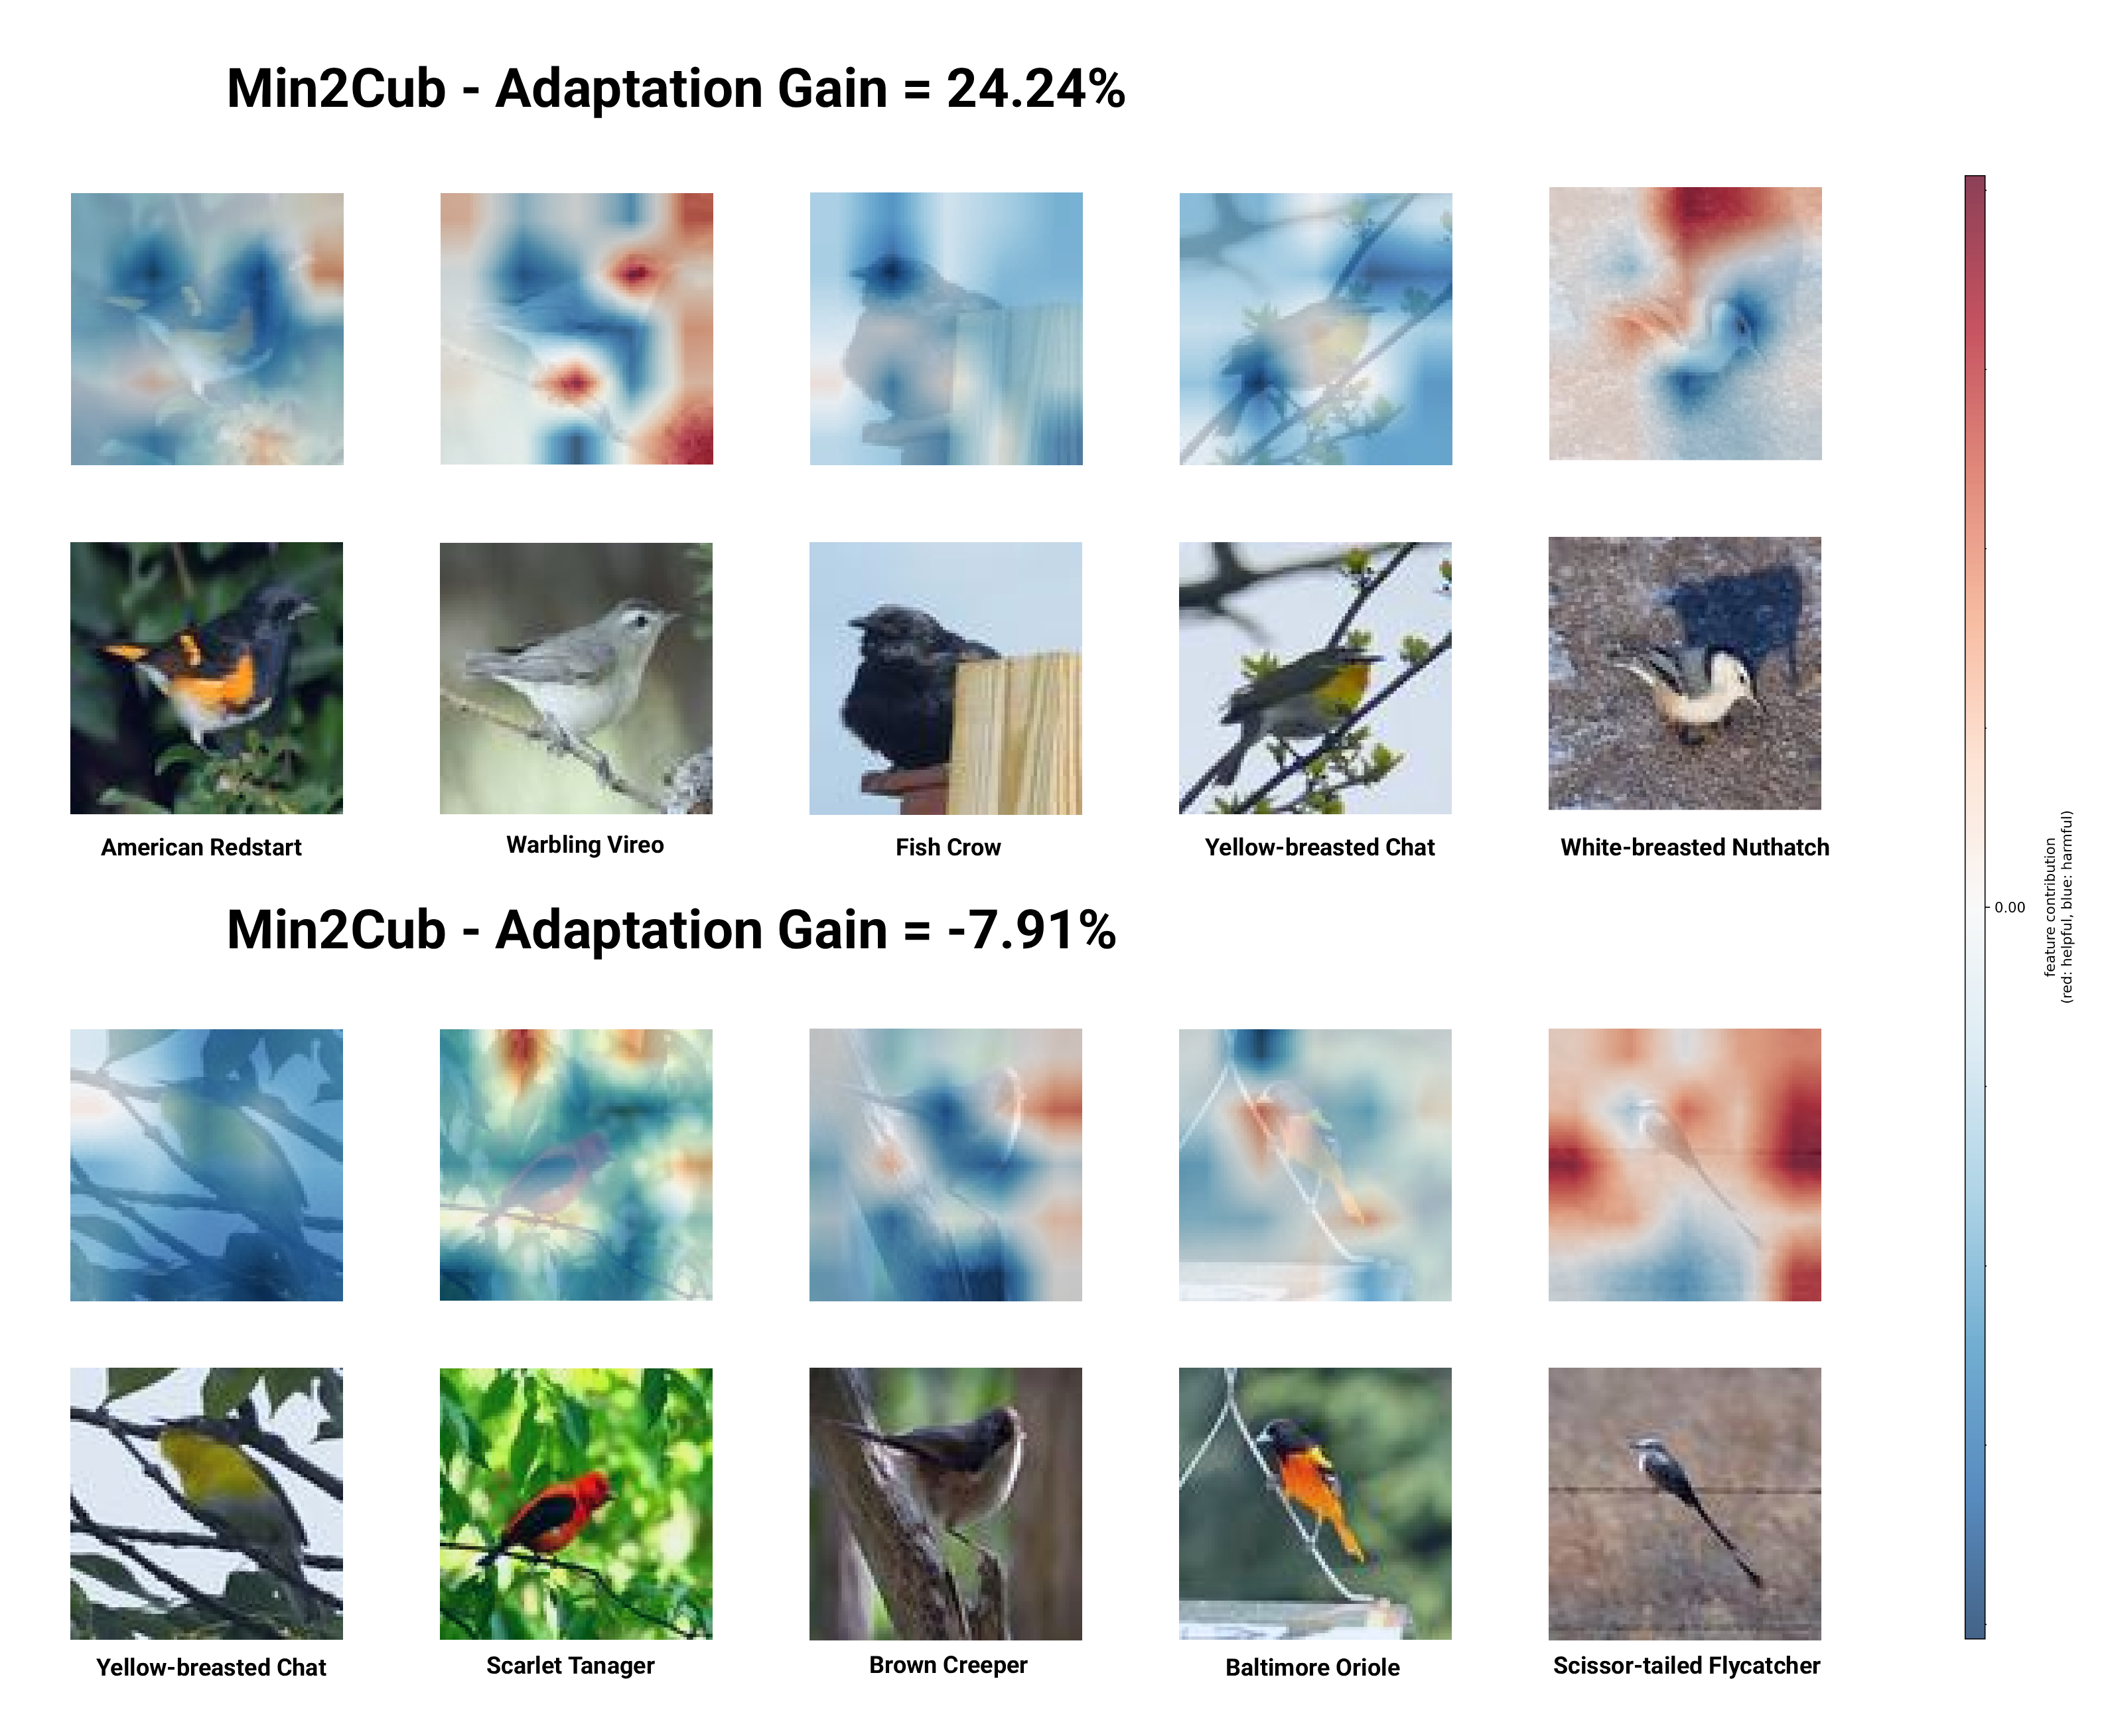
\includegraphics[width=0.95\linewidth]{figures/mini2cub_lmag.png}
    \caption{$\PhiFama$ on the most positive- (top) and most negative-transfer (bottom) mini2cub tasks (red: helpful, blue: harmful). Compare to \Cref{fig:case_study} (tiered2cub): the same contextual-bias and spatial-bleeding patterns appear, at visibly smaller magnitude and extent.}
    \label{fig:supp_mini2cub}
\end{figure*}

\Cref{fig:supp_mini2cub} shows the mini2cub counterpart of \Cref{fig:case_study}. The same three patterns from \Cref{sec:qual_results} recur at smaller magnitude, consistent with miniImageNet's narrower, less category-abstracted prior producing milder adaptation swings than tieredImageNet (\Cref{fig:delta_m_dist}).
